\let\negmedspace\undefined
\let\negthickspace\undefined
\documentclass[journal]{IEEEtran}
\usepackage[a5paper, margin=10mm, onecolumn]{geometry}
%\usepackage{lmodern} % Ensure lmodern is loaded for pdflatex
\usepackage{tfrupee} % Include tfrupee package

\setlength{\headheight}{1cm} % Set the height of the header box
\setlength{\headsep}{0mm}     % Set the distance between the header box and the top of the text

\usepackage{gvv-book}
\usepackage{gvv}
\usepackage{algorithmicx} % Ensure algorithmicx is loaded explicitly
\usepackage{cite}
\usepackage{amsmath,amssymb,amsfonts,amsthm}
\usepackage{graphicx}
\usepackage{textcomp}
\usepackage{xcolor}
\usepackage{txfonts}
\usepackage{listings}
\usepackage{enumitem}
\usepackage{mathtools}
\usepackage{gensymb}
\usepackage{comment}
\usepackage[breaklinks=true]{hyperref}
\usepackage{tkz-euclide} 
\usepackage{listings}
% \usepackage{gvv}                                        
\def\inputGnumericTable{}                                 
\usepackage[latin1]{inputenc}                                
\usepackage{color}                                            
\usepackage{array}                                            
\usepackage{longtable}                                       
\usepackage{calc}                                             
\usepackage{multirow}                                         
\usepackage{hhline}                                           
\usepackage{ifthen}                                           
\usepackage{lscape}
\usepackage{algorithm}
\usepackage{algpseudocode}

\renewcommand{\thefigure}{\theenumi}
\renewcommand{\thetable}{\theenumi}
\setlength{\intextsep}{10pt} % Space between text and floats


\numberwithin{equation}{enumi}
\numberwithin{figure}{enumi}
\renewcommand{\thetable}{\theenumi}

% Marks the beginning of the document
\begin{document}
\bibliographystyle{IEEEtran}

\title{11.16.2.2.5}
\author{EE24BTECH11052 - Rongali Charan}

% \maketitle
% \newpage
% \bigskip
{\let\newpage\relax\maketitle}

\textbf{Question:} A Die is thrown.Describe the following events:\\
E: an even number greater than 4\\

\textbf{Solution:}\\

\begin{enumerate}
    \item \textbf{Total Number of Possible Outcomes}\\
    Let $X$ be the random variable representing the outcome of a single die roll. The sample space is $ S = \cbrak{1, 2, 3, 4, 5, 6}$.  We are interested in the event $E$ where the outcome is an even number greater than 4.  The only outcome satisfying this condition is 6.

    \item \textbf{Probability of Success}\\
    The probability of event $E$ is the number of favorable outcomes divided by the total number of possible outcomes:

$$P(E) = \frac{\text{Number of outcomes in E}}{\text{Total number of outcomes in S}} = \frac{1}{6}$$
    \item \textbf{Defining the Random Variable}\\
    The PMF of the random variable $X$ is given by:

$$P_X(x) = \begin{cases}
    \frac{1}{6}, & x \in \{1, 2, 3, 4, 5, 6\} \\
    0, & \text{otherwise}
\end{cases}$$\\
\textbf{Desired probability} i.e. probability that an even number greater than 4 is when die comes up as 6 
\begin{align} 
     P\brak{X = 6} = \frac{1}{6}
    \end{align}



For the event $E$ (rolling a 6), we can define a new random variable $Y$ such that:\\
    Let $Y$ be the random variable that represents the die turn up to be a 6:
    \begin{align}
        Y &= 1, \text{ If the number is 6, \brak{\text{With probability }p = \frac{1}{6}}}\\
        Y &= 0, \text{ if number gets in \cbrak{1,2,3,4,5}, \brak{\text{With probability } 1 -p = \frac{5}{6}}}
    \end{align}
    \item \textbf{Probability Mass Function (PMF):}\\
    The PMF  of a Bernoulli random variable $Y$ is given by:
    \begin{align}
	P\brak{Y = y} = p^y\brak{1 - p}^{1 - y}, y \in \cbrak{0,1}
    \end{align}
    substituting $p = \frac{1}{6}$,\\
    \begin{align}
     P\brak{Y = 1} = 0.166666, P\brak{Y = 0} = 0.833333
    \end{align}
    \begin{align}
    	P\brak{Y = y} = \begin{cases}
    		0.166666, & y = 1 \\
    		0.833333, & y = 0 \\
    		0, & \text{otherwise}
    	\end{cases}
    \end{align}

    \item \textbf{Cumulative Distribution function (CDF):}\\
    The CDF of a discrete uniform random variable $X$ is:
    \begin{align}
        F_X(k) = P(X \leq k) = \frac{k}{6}, \quad k \in \{1,2,3,4,5,6\}
    \end{align}+

    \begin{align}
        F_X(k) = \begin{cases}
            0, & k < 1 \\
            \frac{k}{6}, & 1 \leq k \leq 6 \\
            1, & k > 6
        \end{cases}
    \end{align}
    The CDF of a Bernoulli random variable Y is defined as:\\
    \begin{align}
    	F_Y\brak{y} = P\brak{Y \leq y}
    \end{align}
    \begin{align}
            F_Y\brak{y} = \begin{cases}
                    0, & y < 0 \\
    \frac{5}{6}, & 0 \leq y < 1 \\
    1, & y \geq 1
            \end{cases}
    \end{align}

\item \textbf{Numerical Solution (Monte Carlo)}\\
We can estimate the probability using the Monte Carlo method.  We simulate a large number of die rolls and count how many times we get a 6.
\end{enumerate}
\begin{figure}[H]
    \centering
    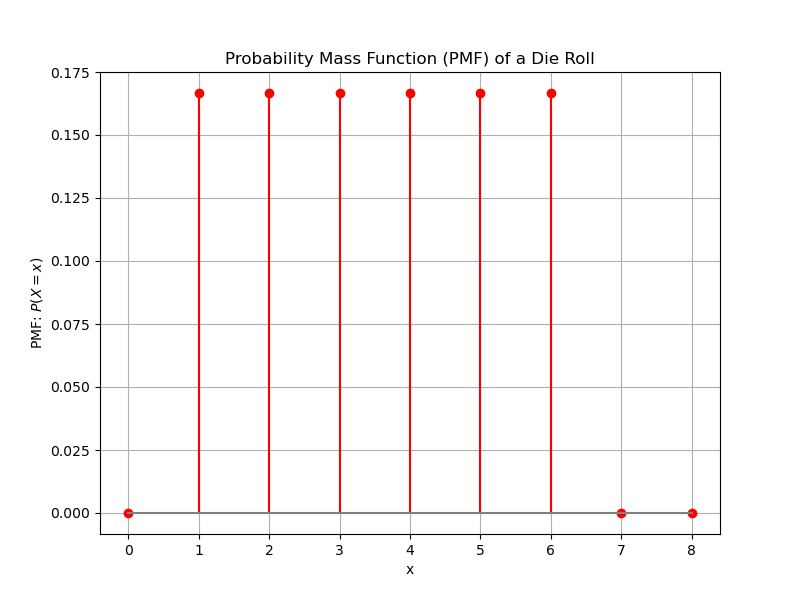
\includegraphics[width=\columnwidth]{figs/pmf_die.png}
    \caption{PMF of the Random Variable}
    \label{fig:enter-label}
\end{figure}

\begin{figure}[H]
    \centering
    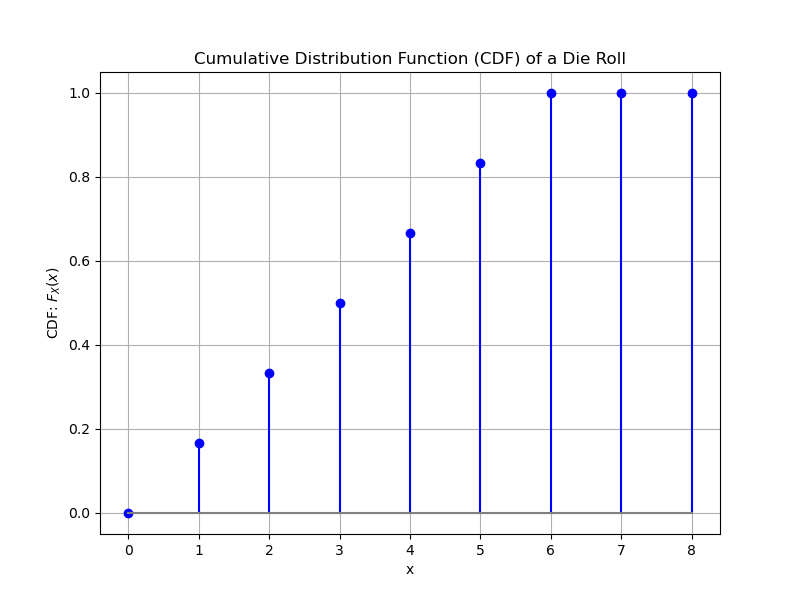
\includegraphics[width=\columnwidth]{figs/cdf_die.png}
    \caption{CDF of the Random Variable}
    \label{fig:enter-label}
\end{figure}
\end{document}i
